\chapter{Моделирование проблемной области}
\label{chapter2}

\section{Построение фрагмента поля знаний на естественном языке}

В данном разделе приводится фрагмент полуформализованного описания проблемной области (фрагменты поля знаний) в виде совокупности конструкций вида: \enquote{ЕСЛИ \dots{} ТО \dots{}} на естественном языке, полученное в результате исследования данной проблемной области.

\begin{enumerate}
    \item Если на листьях появились жёлто-зелёные угловатые пятна и наблюдается серо-фиолетовый налёт на нижней стороне листьев, и влажность воздуха выше \SI{80}{\percent}, и температура воздуха ниже \SI{20}{\degree C}, то диагностировать \enquote{пероноспороз}.

    \item Если на стеблях и листьях наблюдается белый мучнистый налёт и листья закручиваются и становятся коричневыми, и влажность воздуха не менее \SI{50}{\percent}, и температура воздуха в диапазоне \SIrange{15}{25}{\degree C}, то диагностировать \enquote{мучнистая роса}.

    \item Если на нижней стороне листьев появился белый налёт, и влажность воздуха не менее \SI{50}{\percent}, и температура воздуха в диапазоне \SIrange{15}{25}{\degree C}, то диагностировать \enquote{мучнистая роса}.

    \item Если на нижней стороне листьев наблюдается серый налёт, и влажность воздуха выше \SI{80}{\percent}, и температура воздуха ниже \SI{20}{\degree C}, то диагностировать \enquote{ложная мучнистая роса (пероноспороз)}.

    \item Если на листьях появились жёлто-коричневые пятна с чёткой каймой и на стеблях образовались вдавленные овальные язвочки жёлто-коричневого цвета, и температура воздуха не менее \SI{20}{\degree C}, и влажность воздуха не менее \SI{80}{\percent}, то диагностировать \enquote{антракноз}.

    \item Если на листьях появились обширные пятна, и температура воздуха не менее \SI{20}{\degree C}, и влажность воздуха не менее \SI{80}{\percent}, то диагностировать \enquote{антракноз}.

    \item Если растение увядает, и листья желтеют от основания к верхушке, и корневая шейка темнеет, то диагностировать \enquote{фузариозное увядание}.

    \item Если растение увядает сильно и корни приобретают чёрный цвет, то диагностировать \enquote{фузариоз}.

    \item Если нижние листья становятся бледно-зелёными и содержание азота в почве критическое (уровень 0) и рост растения замедляется, то диагностировать \enquote{дефицит азота}.

    \item Если листья полностью пожелтели и содержание азота в почве менее 50 мг/кг, то диагностировать \enquote{дефицит азота}.

    \item Если листья приобретают тёмно-зелёную окраску с фиолетовым оттенком и содержание фосфора в почве критическое (уровень 0), то диагностировать \enquote{дефицит фосфора}.

    \item Если края листьев буреют и появляется краевой ожог и содержание калия в почве критическое (уровень 0), то диагностировать \enquote{дефицит калия}.

    \item Если между жилками старых листьев развивается хлороз и содержание магния в почве неоптимально (уровень 1), то диагностировать \enquote{дефицит магния}.

    \item Если между жилками старых листьев развивается интенсивный хлороз и содержание магния в почве менее 50 мг/кг и pH почвы щелочной (выше 7.5), то диагностировать \enquote{дефицит магния}.

    \item Если между жилками молодых листьев развивается хлороз и содержание железа в почве критическое (уровень 0), то диагностировать \enquote{дефицит железа}.

    \item Если между жилками молодых листьев развивается интенсивный хлороз и содержание железа в почве менее 10 мг/кг и pH почвы щелочной (выше 7.5), то диагностировать \enquote{дефицит железа}.

    \item Если листья сильно закручиваются и содержание магния в почве критическое (уровень 0), то диагностировать \enquote{тяжёлый дефицит магния}.

    \item Если жилки листьев зеленоватые и содержание магния в почве неоптимально (уровень 1), то диагностировать \enquote{лёгкий дефицит магния}.

    \item Если лист зелёный и на нём отсутствуют пятна, то состояние листа \enquote{здоровое}.

    \item Если лист жёлтый и на нём появились коричневые круглые пятна, то состояние листа \enquote{подозрение на заболевание}.

    \item Если лист имеет мучнистую текстуру и покрыт белым налётом, то состояние листа \enquote{обнаружена мучнистая роса}.

    \item Если края листа некротизированы (бурые) и текстура листа хрупкая, то состояние листа \enquote{тяжёлый дефицит питательных веществ}.

    \item Если нижняя сторона листа покрыта серым налётом и лист бледно-жёлтый, то состояние листа \enquote{обнаружена ложная мучнистая роса}.

    \item Если между жилками листа развивается хлороз (обесцвечивание) и жилки остаются зелёными, то состояние листа \enquote{дефицит микроэлементов}.

    \item Если на листе появились жёлтые пятна с жёлтым ореолом и пятна имеют концентрические кольца, то состояние листа \enquote{обнаружен антракноз}.

    \item Если лист увядает и приобретает тёмно-коричневый цвет, то состояние листа \enquote{подозрение на фузариоз}.

    \item Если лист имеет высокую влажность (покрыт росой) и воздух имеет высокую влажность и текстура листа мягкая, то состояние листа \enquote{риск грибковой инфекции}.

    \item Если лист старый и его цвет бледный, то состояние листа \enquote{нормальное старение}.

    \item Если высота растения нормальная и листья здоровые и стебель прочный, то состояние растения \enquote{активный рост}.

    \item Если высота растения остаётся позади в развитии и листья пожелтели, то состояние растения \enquote{наличие дефицита питательных веществ}.

    \item Если растение сильно увядает и стебель мягкий и корни чёрного цвета, то состояние растения \enquote{критическое корневое заболевание}.

    \item Если диагностирована мучнистая роса и состояние листа \enquote{обнаружена мучнистая роса}, то состояние растения \enquote{грибковое заболевание}.

    \item Если диагностирован антракноз и на листьях обширные пятна, то состояние растения \enquote{тяжёлое заболевание}.

    \item Если диагностирован дефицит азота и содержание азота в почве критическое, то состояние растения \enquote{азотное голодание}.

    \item Если высота растения нормальная и листья здоровые и состояние почвы отличное, то состояние растения \enquote{оптимальный рост}.

    \item Если на стебле присутствуют поражения (язвочки) и стебель бурый и обесцвечен, то состояние растения \enquote{стеблевое заболевание}.

    \item Если плод деформирован и диагностирован фузариоз, то состояние растения \enquote{нарушение плодоношения}.

    \item Если влажность почвы выше нормы (уровень 2) и содержание калия оптимально (уровень \geq 1) и содержание азота оптимально (уровень \geq 1), то состояние почвы \enquote{удовлетворительное}.

    \item Если влажность почвы высокая (уровень 2) и содержание калия оптимально (уровень 2) и содержание азота оптимально (уровень 2) и содержание магния оптимально (уровень 2), то состояние почвы \enquote{отличное}.

    \item Если влажность почвы высокая (уровень 2) и содержание магния неоптимально (уровень 1) и содержание азота оптимально (уровень 2), то состояние почвы \enquote{хорошее}.

    \item Если влажность почвы высокая (уровень 2) и содержание калия оптимально (уровень 2) и содержание азота неоптимально (уровень 1), то состояние почвы \enquote{хорошее}.

    \item Если влажность почвы низкая (уровень 0) и содержание калия оптимально (уровень 2) и содержание азота оптимально (уровень 2), то состояние почвы \enquote{удовлетворительное}.

    \item Если влажность почвы высокая (уровень 2) и содержание калия критическое (уровень 0) и содержание азота критическое (уровень 0) и содержание магния критическое (уровень 0), то состояние почвы \enquote{удовлетворительное}.

    \item Если влажность почвы высокая (уровень 2) и содержание азота критическое (уровень 0), то состояние почвы \enquote{неудовлетворительное}.

    \item Если влажность почвы высокая (уровень 2) и содержание магния критическое (уровень 0), то состояние почвы \enquote{неудовлетворительное}.

    \item Если влажность почвы низкая или критическая (уровень \leq 1) и содержание калия критическое (уровень 0) и содержание азота критическое (уровень 0) и содержание магния критическое (уровень 0), то состояние почвы \enquote{неудовлетворительное}.

    \item Если температура воздуха критическая (уровень 0) и влажность воздуха критическая (уровень 0), то состояние воздуха \enquote{критическое}.

    \item Если температура воздуха неоптимальная (уровень 1) и влажность воздуха оптимальна (уровень 2), то состояние воздуха \enquote{благоприятное}.

    \item Если температура воздуха оптимальна (уровень 2) и влажность воздуха оптимальна (уровень 2), то состояние воздуха \enquote{очень благоприятное}.

    \item Если содержание азота в почве критическое (уровень 0) и влажность почвы выше нормы (уровень 1), то состояние питания \enquote{критическое с риском вымывания}.

    \item Если содержание азота в почве неоптимально (уровень 1) и содержание калия в почве неоптимально (уровень 1) и содержание фосфора в почве неоптимально (уровень 1), то состояние питания \enquote{нестабильное}.

    \item Если содержание азота в почве оптимально (уровень 2) и содержание калия в почве оптимально (уровень 2) и содержание фосфора в почве оптимально (уровень 2), то состояние питания \enquote{стабильное}.

    \item Если диагностирована мучнистая роса и влажность воздуха высокая и температура воздуха умеренная (\SIrange{16}{20}{\degree C}), то выдать рекомендацию \enquote{обработать посадки коллоидной серой, соблюдать севооборот}.

    \item Если диагностирован пероноспороз и влажность почвы выше нормы (уровень 1), то выдать рекомендацию \enquote{обработать бордоской жидкостью, прогреть семена при \SI{45}{\degree C} в течение 2 часов}.

    \item Если диагностирован антракноз и температура воздуха высокая (\SIrange{24}{25}{\degree C}) и влажность воздуха выше \SI{60}{\percent}, то выдать рекомендацию \enquote{удалить пораженные части растений, обработать фунгицидами}.

    \item Если диагностировано фузариозное увядание, то выдать рекомендацию \enquote{удалить пораженные растения, продезинфицировать почву, соблюдать севооборот минимум 4 года}.

    \item Если диагностирован фузариоз, то выдать рекомендацию \enquote{удалить пораженные растения, продезинфицировать почву, избегать избыточной влажности}.

    \item Если диагностирована ложная мучнистая роса, то выдать рекомендацию \enquote{обработать медьсодержащими фунгицидами, улучшить вентиляцию, снизить влажность}.

    \item Если диагностирован дефицит азота и состояние питания нестабильное, то выдать рекомендацию \enquote{внести азотные удобрения (мочевина, аммиачная селитра), провести листовую подкормку 2\% раствором нитрата кальция}.

    \item Если диагностирован дефицит калия и содержание калия в почве критическое (уровень 0), то выдать рекомендацию \enquote{внести калийные удобрения, избегать избыточного азотного питания}.

    \item Если диагностирован дефицит магния, то выдать рекомендацию \enquote{провести внекорневую подкормку сульфатом магния}.

    \item Если диагностирован тяжёлый дефицит магния, то выдать рекомендацию \enquote{срочная внекорневая подкормка сульфатом магния 10\% раствором}.

    \item Если диагностирован лёгкий дефицит магния, то выдать рекомендацию \enquote{внекорневая подкормка сульфатом магния 5\% раствором, внесение органических удобрений}.

    \item Если диагностирован дефицит железа и pH почвы выше 7.5, то выдать рекомендацию \enquote{провести внекорневую подкормку хелатом железа, снизить pH почвы}.

    \item Если диагностирован дефицит фосфора, то выдать рекомендацию \enquote{внести фосфорные удобрения, улучшить усвояемость путем внесения органических удобрений}.
\end{enumerate}


\subsection{Правила на языке представления знаний системы G2}

\begin{lstlisting}[language=C, breaklines=true, breakatwhitespace=false]
unconditionally start detect_magnesium_deficiency(leaf1, soil1, plant1)
unconditionally start show_lights()
unconditionally start show_lights_diagnoz(plant1, air1, soil1)
unconditionally start constraints(air1, soil1, plant1)
unconditionally start simulate_day(air1, soil1, plant1)
initially start initialize_simulation()
    
for any soil soil1
    when the soil_humidity_state of soil1 = 1
    and the soil_potassium_state of soil1 >= 1
    and the soil_nitrogen_state of soil1 >= 1
    then conclude that the soil_state of soil1 = "satisfactory"

for any soil soil1
    when the soil_humidity_state of soil1 = 2
    and the soil_potassium_state of soil1 = 2
    and the soil_nitrogen_state of soil1 = 2
    and the soil_magnesium_state of soil1 = 2
    then conclude that the soil_state of soil1 = "excellent"

for any soil soil1
    when the soil_humidity_state of soil1 = 2
    and the soil_magnesium_state of soil1 = 1
    and the soil_nitrogen_state of soil1 = 2
    then conclude that the soil_state of soil1 = "good"

for any soil soil1
    when the soil_humidity_state of soil1 = 2
    and the soil_potassium_state of soil1 = 2
    and the soil_nitrogen_state of soil1 = 1
    then conclude that the soil_state of soil1 = "good"

for any soil soil1
    when the soil_humidity_state of soil1 = 0
    and the soil_potassium_state of soil1 = 2
    and the soil_nitrogen_state of soil1 = 2
    then conclude that the soil_state of soil1 = "satisfactory"

for any soil soil1
    when the soil_humidity_state of soil1 = 2
    and the soil_potassium_state of soil1 = 0
    and the soil_nitrogen_state of soil1 = 0
    and the soil_magnesium_state of soil1 = 0
    then conclude that the soil_state of soil1 = "satisfactory"

for any soil soil1
    when the soil_humidity_state of soil1 = 2
    and the soil_nitrogen_state of soil1 = 0
    then conclude that the soil_state of soil1 = "unsatisfactory"

for any soil soil1
    when the soil_humidity_state of soil1 = 2
    and the soil_magnesium_state of soil1 = 0
    then conclude that the soil_state of soil1 = "unsatisfactory"

for any soil soil1
    when the soil_humidity_state of soil1 <= 1
    and the soil_potassium_state of soil1 = 0
    and the soil_nitrogen_state of soil1 = 0
    and the soil_magnesium_state of soil1 = 0
    then conclude that the soil_state of soil1 = "unsatisfactory"

for any air air1
    when the air_temperature_state of air1 = 0
    and the air_humidity_state of air1 = 0
    then conclude that the air_state of air1 = "critical"

for any air air1
    when the air_temperature_state of air1 = 1
    and the air_humidity_state of air1 = 2
    then conclude that the air_state of air1 = "friendly"

for any air air1
    when the air_temperature_state of air1 = 2
    and the air_humidity_state of air1 = 2
    then conclude that the air_state of air1 = "ultrafriendly"

for any plant plant1 for any air air1
    when the leaf_spots_state of plant1 = "yellow-green-angular"
    and the leaf_underside_coating of plant1 = "gray-violet"
    and the air_humidity_state of air1 > 80
    and the air_temperature_state of air1 < 20
    then conclude that the disease_diagnosis of plant1 = "peronosporosis"

for any plant plant1 for any air air1
    when the leaf_stem_coating of plant1 = "white-powdery"
    and the leaf_curl_state of plant1 = "curled-brown"
    and the air_humidity_state of air1 >= 50
    and the air_temperature_state of air1 >= 15
    and the air_temperature_state of air1 <= 25
    then conclude that the disease_diagnosis of plant1 = "powdery_mildew"

for any plant plant1 for any air air1
    when the leaf_underside_coating of plant1 = "white"
    and the air_humidity_state of air1 >= 50
    and the air_temperature_state of air1 >= 15
    and the air_temperature_state of air1 <= 25
    then conclude that the disease_diagnosis of plant1 = "powdery_mildew"

for any plant plant1 for any air air1
    when the leaf_underside_coating of plant1 = "gray"
    and the air_humidity_state of air1 > 80
    and the air_temperature_state of air1 < 20
    then conclude that the disease_diagnosis of plant1 = "downy_mildew"

for any plant plant1 for any air air1
    when the leaf_spots_state of plant1 = "yellow-brown-bordered"
    and the stem_lesions of plant1 = "depressed-oval-yellow-brown"
    and the air_temperature_state of air1 >= 20
    and the air_humidity_state of air1 >= 80
    then conclude that the disease_diagnosis of plant1 = "anthracnose"

for any plant plant1 for any air air1
    when the leaf_spots_state of plant1 = "extensive"
    and the air_temperature_state of air1 >= 20
    and the air_humidity_state of air1 >= 80
    then conclude that the disease_diagnosis of plant1 = "anthracnose"

for any plant plant1
    when the plant_wilting of plant1 = "wilted"
    and the leaf_yellowing_pattern of plant1 = "base-to-top"
    and the root_collar_state of plant1 = "darkened"
    then conclude that the disease_diagnosis of plant1 = "fusarium_wilt"

for any plant plant1
    when the plant_wilting of plant1 = "strong"
    and the root_color_state of plant1 = "black"
    then conclude that the disease_diagnosis of plant1 = "fusariosis"

for any plant plant1 for any soil soil1
    when the lower_leaves_color of plant1 = "pale-green"
    and the soil_nitrogen_state of soil1 = 0
    and the growth_rate of plant1 = "slowed"
    then conclude that the deficiency_diagnosis of plant1 = "nitrogen_deficiency"

for any plant plant1
    when the leaf_yellowing_pattern of plant1 = "complete"
    and the soil_nitrogen_state of plant1 < 50
    then conclude that the deficiency_diagnosis of plant1 = "N"

for any plant plant1 for any soil soil1
    when the leaf_color_tone of plant1 = "dark-green-purple"
    and the soil_phosphorus_state of soil1 = 0
    then conclude that the deficiency_diagnosis of plant1 = "phosphorus_deficiency"

for any plant plant1 for any soil soil1
    when the leaf_edge_state of plant1 = "brown-burned"
    and the soil_potassium_state of soil1 = 0
    then conclude that the deficiency_diagnosis of plant1 = "potassium_deficiency"

for any plant plant1 for any soil soil1
    when the old_leaf_interveinal_chlorosis of plant1 = "present"
    and the soil_magnesium_state of soil1 = 1
    then conclude that the deficiency_diagnosis of plant1 = "magnesium_deficiency"

for any plant plant1 for any soil soil1
    when the old_leaf_interveinal_chlorosis of plant1 = "strong"
    and the soil_magnesium_state of soil1 < 50
    and the soil_ph_state of soil1 = "alkaline"
    then conclude that the deficiency_diagnosis of plant1 = "Mg"

for any plant plant1 for any soil soil1
    when the young_leaf_interveinal_chlorosis of plant1 = "present"
    and the soil_iron_state of soil1 = 0
    then conclude that the deficiency_diagnosis of plant1 = "iron_deficiency"

for any plant plant1 for any soil soil1
    when the young_leaf_interveinal_chlorosis of plant1 = "strong"
    and the soil_iron_state of soil1 < 10
    and the soil_ph_state of soil1 = "alkaline"
    then conclude that the deficiency_diagnosis of plant1 = "Fe"

for any plant plant1 for any soil soil1
    when the leaf_curl_state of plant1 = "strong_curl"
    and the soil_magnesium_state of soil1 = 0
    then conclude that the deficiency_diagnosis of plant1 = "magnesium_severe"

for any plant plant1 for any soil soil1
    when the leaf_vein_color of plant1 = "greenish"
    and the soil_magnesium_state of soil1 = 1
    then conclude that the deficiency_diagnosis of plant1 = "magnesium_mild"

for any leaf leaf1 for any plant plant1
    when the leaf_color of leaf1 = "green"
    and the leaf_spots of leaf1 = "none"
    then conclude that the leaf_state of leaf1 = "healthy"

for any leaf leaf1 for any plant plant1
    when the leaf_color of leaf1 = "yellow"
    and the leaf_spots of leaf1 = "brown-circular"
    then conclude that the leaf_state of leaf1 = "disease_suspected"

for any leaf leaf1 for any plant plant1
    when the leaf_texture of leaf1 = "powdery"
    and the leaf_color of leaf1 = "white-coated"
    then conclude that the leaf_state of leaf1 = "powdery_mildew_present"

for any leaf leaf1 for any plant plant1
    when the leaf_margin_state of leaf1 = "brown-necrotic"
    and the leaf_texture of leaf1 = "brittle"
    then conclude that the leaf_state of leaf1 = "severe_nutrient_deficiency"

for any leaf leaf1 for any plant plant1
    when the leaf_underside of leaf1 = "gray-coating"
    and the leaf_color of leaf1 = "pale-yellow"
    then conclude that the leaf_state of leaf1 = "downy_mildew_present"

for any leaf leaf1 for any plant plant1
    when the leaf_interveinal_area of leaf1 = "chlorotic"
    and the leaf_veins of leaf1 = "green"
    then conclude that the leaf_state of leaf1 = "micronutrient_deficiency"

for any leaf leaf1 for any plant plant1
    when the leaf_spots of leaf1 = "yellow-halo"
    and the leaf_spots of leaf1 = "concentric-rings"
    then conclude that the leaf_state of leaf1 = "anthracnose_present"

for any leaf leaf1 for any plant plant1
    when the leaf_wilting of leaf1 = "present"
    and the leaf_color of leaf1 = "dark-brown"
    then conclude that the leaf_state of leaf1 = "fusarium_suspected"

for any leaf leaf1 for any plant plant1 for any air air1
    when the leaf_moisture of leaf1 = "high"
    and the air_humidity_state of air1 = "high"
    and the leaf_texture of leaf1 = "soft"
    then conclude that the leaf_state of leaf1 = "fungal_infection_risk"

for any leaf leaf1
    when the leaf_age of leaf1 = "old"
    and the leaf_color of leaf1 = "pale"
    then conclude that the leaf_state of leaf1 = "senescence_normal"

for any plant plant1
    when the plant_height of plant1 = "normal"
    and the leaf_state of plant1 = "healthy"
    and the stem_state of plant1 = "firm"
    then conclude that the plant_state of plant1 = "vigorous"

for any plant plant1
    when the plant_height of plant1 = "stunted"
    and the leaf_state of plant1 = "yellowing"
    then conclude that the plant_state of plant1 = "nutrient_deficiency_present"

for any plant plant1
    when the plant_wilting of plant1 = "severe"
    and the stem_state of plant1 = "soft"
    and the root_color_state of plant1 = "black"
    then conclude that the plant_state of plant1 = "root_disease_critical"

for any plant plant1
    when the disease_diagnosis of plant1 = "powdery_mildew"
    and the leaf_state of plant1 = "powdery_mildew_present"
    then conclude that the plant_state of plant1 = "diseased_fungal"

for any plant plant1
    when the disease_diagnosis of plant1 = "anthracnose"
    and the leaf_spots of plant1 = "extensive"
    then conclude that the plant_state of plant1 = "heavily_diseased"

for any plant plant1 for any soil soil1
    when the deficiency_diagnosis of plant1 = "nitrogen_deficiency"
    and the soil_nitrogen_state of soil1 = 0
    then conclude that the plant_state of plant1 = "nitrogen_starved"

for any plant plant1 for any soil soil1
    when the plant_height of plant1 = "normal"
    and the leaf_state of plant1 = "healthy"
    and the soil_state of soil1 = "excellent"
    then conclude that the plant_state of plant1 = "optimal_growth"

for any plant plant1
    when the stem_state of plant1 = "lesions-present"
    and the stem_color of plant1 = "brown-discolored"
    then conclude that the plant_state of plant1 = "stem_disease_present"

for any plant plant1
    when the fruit_state of plant1 = "deformed"
    and the disease_diagnosis of plant1 = "fusariosis"
    then conclude that the plant_state of plant1 = "fruit_production_compromised"

for any soil soil1
    when the soil_nitrogen_state of soil1 = 0
    and the soil_humidity_state of soil1 = 1
    then conclude that the nutrition_state of soil1 = "critical_with_leaching_risk"

for any soil soil1
    when the soil_nitrogen_state of soil1 = 1
    and the soil_potassium_state of soil1 = 1
    and the soil_phosphorus_state of soil1 = 1
    then conclude that the nutrition_state of soil1 = "unstable"

for any soil soil1
    when the soil_nitrogen_state of soil1 = 2
    and the soil_potassium_state of soil1 = 2
    and the soil_phosphorus_state of soil1 = 2
    then conclude that the nutrition_state of soil1 = "stable"

for any plant plant1 for any air air1 for any display_object display1
    when the disease_diagnosis of plant1 = "powdery_mildew"
    and the air_humidity_state of air1 = "high"
    and the air_temperature_state of air1 = "moderate_16_20"
    then conclude that the recommendation of display1 = "обработать посадки коллоидной серой, соблюдать севооборот"

for any plant plant1 for any soil soil1 for any display_object display1
    when the disease_diagnosis of plant1 = "peronosporosis"
    and the soil_humidity_state of soil1 = 1
    then conclude that the recommendation of display1 = "обработать бордоской жидкостью, прогреть семена при 45C в течение 2 часов"

for any plant plant1 for any air air1 for any display_object display1
    when the disease_diagnosis of plant1 = "anthracnose"
    and the air_temperature_state of air1 = "high_24_25"
    and the air_humidity_state of air1 = "above_60%"
    then conclude that the recommendation of display1 = "удалить пораженные части растений, обработать фунгицидами"

for any plant plant1 for any display_object display1
    when the disease_diagnosis of plant1 = "fusarium_wilt"
    then conclude that the recommendation of display1 = "удалить пораженные растения, продезинфицировать почву, соблюдать севооборот минимум 4 года"

for any plant plant1 for any display_object display1
    when the disease_diagnosis of plant1 = "fusariosis"
    then conclude that the recommendation of display1 = "удалить пораженные растения, продезинфицировать почву, избегать избыточной влажности"

for any plant plant1 for any display_object display1
    when the disease_diagnosis of plant1 = "downy_mildew"
    then conclude that the recommendation of display1 = "обработать медьсодержащими фунгицидами, улучшить вентиляцию, снизить влажность"

for any plant plant1 for any soil soil1 for any display_object display1
    when the deficiency_diagnosis of plant1 = "nitrogen_deficiency"
    and the nutrition_state of soil1 = "unstable"
    then conclude that the recommendation of display1 = "внести азотные удобрения (мочевина, аммиачная селитра), провести листовую подкормку 2% раствором нитрата кальция"

for any plant plant1 for any soil soil1 for any display_object display1
    when the deficiency_diagnosis of plant1 = "potassium_deficiency"
    and the soil_potassium_state of soil1 = 0
    then conclude that the recommendation of display1 = "внести калийные удобрения, избегать избыточного азотного питания"

for any plant plant1 for any display_object display1
    when the deficiency_diagnosis of plant1 = "magnesium_deficiency"
    then conclude that the recommendation of display1 = "провести внекорневую подкормку сульфатом магния"

for any plant plant1 for any display_object display1
    when the deficiency_diagnosis of plant1 = "magnesium_severe"
    then conclude that the recommendation of display1 = "срочная внекорневая подкормка сульфатом магния 10% раствором"

for any plant plant1 for any display_object display1
    when the deficiency_diagnosis of plant1 = "magnesium_mild"
    then conclude that the recommendation of display1 = "внекорневая подкормка сульфатом магния 5% раствором, внесение органических удобрений"

for any plant plant1 for any soil soil1 for any display_object display1
    when the deficiency_diagnosis of plant1 = "iron_deficiency"
    and the soil_ph_state of soil1 = "above_7_5"
    then conclude that the recommendation of display1 = "провести внекорневую подкормку хелатом железа, снизить pH почвы"

for any plant plant1 for any soil soil1 for any display_object display1
    when the deficiency_diagnosis of plant1 = "phosphorus_deficiency"
    then conclude that the recommendation of display1 = "внести фосфорные удобрения, улучшить усвояемость путем внесения органических удобрений"
\end{lstlisting}
    

\section{Построение имитационной модели, используемой в прототипе ИЭС}

\begin{figure}[H]
    \centering
    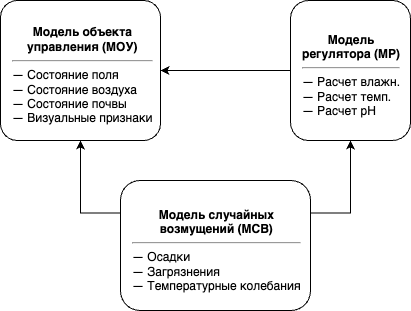
\includegraphics[width=0.5\textwidth]{img/im_model.png}
    \caption{Имитационная модель.}
    \label{fig:im_model}
\end{figure}

Система G2 не имеет встроенной подсистемы имитационного моделирования, поэтому имитационная модель и средства её отладки реализуются базовыми средствами системы G2, а именно правилами и процедурами G2.

Для реализации прототипа была построена имитационная модель (ИМ), состав которой представлен ниже.

\subsection{Состав имитационной модели}

В качестве метода имитационного моделирования выбран подход \textbf{сканирования активностей}. Для этого выделяются состояния системы и описываются действия, которые переводят ее из одного состояния в другое. Условия начала или окончания действия проверяются после очередного продвижения имитационного времени. Если заданные условия удовлетворяются, происходит соответствующее действие. Для того чтобы было выполнено каждое действие в модели, сканирование условий производится для всего множества действий при каждом продвижении имитационного времени. Время изменения состояния поля составляет постоянную величину, которая сопоставляется с интервалом сканирования активности.

\subsection{Параметры модели}

Вектор $Z(T)$ --- множество выходных параметров модели объекта управления, которые затем поступают на вход в экспертную систему.

Вектор $E(T)$ --- указывает на множество возмущений.

Вектор $U(T)$ --- множество контролируемых управляемых входов, которые поступают в модель объекта управления от модели регулятора.

Вектор $Y(T)$ --- множество выходных параметров объекта управления, использующихся в модели регулятора.

Вектор $X(T)$ --- множество контролируемых неуправляемых входов, которые поступают в модель объекта управления.

\subsection{Конкретизация теоретико-множественного представления}

Имитационная модель представляется в виде:
\[M_{\text{им}} = \langle \text{МОУ, МР, МСВ, } V_x, V_u, V_y, V_e, V_z, S, F_{xeu \to yz}, F_{y \to u} \rangle,\]
где:

\begin{description}
    \item[МОУ] --- модель объекта управления ($\langle A1, A2, A3 \rangle$).
    \item[МР] --- модель регулятора ($\langle B1, B2, B3, B4, B5, B6 \rangle$).
    \item[МСВ] --- модель случайных возмущений ($\{C1, C2\}$).
\end{description}

\subsection{Преобразование численных переменных в символьные}

Для передачи данных в базу знаний используется процедура перевода численных значений параметров в символьные категории (фаззификация).

\begin{table}[H]
\centering
\caption{Диапазоны для перевода численных переменных в символьные}
\label{tab:ranges}
\begin{tabularx}{\textwidth}{|X|c|c|c|}
\hline
\textbf{Параметр} & \textbf{Критическое} & \textbf{Неоптимальное} & \textbf{Оптимальное} \\ \hline
Температура воздуха, \SI{}{\degree C} & $< \num{10}$ или $> \num{35}$ & \num{10}--\num{16}, \num{26}--\num{35} & \num{16}--\num{26} \\ \hline
Влажность воздуха, \SI{}{\percent} & $< \num{40}$ или $> \num{80}$ & \num{40}--\num{50}, \num{70}--\num{80} & \num{50}--\num{70} \\ \hline
Влажность почвы, \SI{}{\percent} & $< \num{60}$ или $> \num{90}$ & \num{60}--\num{70}, \num{85}--\num{90} & \num{70}--\num{85} \\ \hline
Азот (N), \SI{}{\percent} & $< \num{1.5}$ & \num{1.5}--\num{2.5} & \num{2.5}--\num{4.0} \\ \hline
Фосфор (P), \SI{}{\percent} & $< \num{0.3}$ & \num{0.3}--\num{0.5} & \num{0.5}--\num{0.8} \\ \hline
Калий (K), \SI{}{\percent} & $< \num{1.0}$ & \num{1.0}--\num{1.5} & \num{1.5}--\num{2.5} \\ \hline
pH почвы & $< \num{6.0}$ или $> \num{7.5}$ & \num{6.0}--\num{6.2}, \num{7.2}--\num{7.5} & \num{6.2}--\num{7.2} \\ \hline
\end{tabularx}
\end{table}

\subsection{Конкретизация этапов имитационного эксперимента}

Согласно методологии построения динамических интегрированных экспертных систем, существует \num{9} этапов имитационного эксперимента, среди которых:
\begin{enumerate}
    \item Формулировка проблемы и целей имитационного эксперимента.
    \item Определение релевантных ресурсов и законов функционирования моделируемой системы; формализация моделируемой системы.
    \item Программирование имитационной модели.
    \item Планирование имитационных экспериментов, определение начальных условий.
    \item Получение исходных данных.
    \item Проведение имитационных экспериментов.
    \item Обработка результатов экспериментов.
    \item Интерпретация полученных данных.
\end{enumerate}

В рамках настоящей работы данные пункты приобретают следующий смысл:

\subsubsection{Цель имитационного эксперимента}

Целью имитационного моделирования является проверка действий прототипа динамической интегрированной экспертной системы в зависимости от различных условий, возникающих во внешней среде и влияющих на содержание питательных веществ в почве, с дальнейшей интерпретацией полученных результатов.

\subsubsection{Цель имитационного эксперимента}

Целью имитационного моделирования является исследование динамики внешней среды сада при различных внешних воздействиях и анализ граничных значений параметров окружающей среды (температура, влажность, pH почвы, содержание питательных веществ), частоты и характера их колебаний, влияния на визуальные признаки растений дынь и оценка адекватности разработанной базы знаний экспертной системы при обработке результатов имитации.


\subsubsection{Законы функционирования}

Законы функционирования моделируемой системы составляют совокупность правил и процедур, представленные в разделе 2.1.

В рамках данной работы было принято решение о необходимости проведения следующих имитационных экспериментов:
\begin{itemize}
    \item \textbf{Эксперимент \num{1}:} Моделирование нестабильного содержания азота в почве при различных уровнях осадков и анализ развития визуальных признаков азотного голодания и динамики пожелтения листьев.
    \item \textbf{Эксперимент \num{2}:} Моделирование одновременного дефицита нескольких макроэлементов (NPK) и оценка комплексного влияния на визуальное состояние растений дынь, выявление граничных значений содержания элементов.
    \item \textbf{Эксперимент \num{3}:} Моделирование благоприятных условий для развития грибковых заболеваний (мучнистая роса, пероноспороз, антракноз) при различных комбинациях температуры и влажности воздуха, определение пороговых значений этих параметров.
    \item \textbf{Эксперимент \num{4}:} Моделирование колебаний pH почвы и последующего развития дефицита микроэлементов (железа, магния), установление связи между щелочностью почвы и визуальными симптомами хлороза.
    \item \textbf{Эксперимент \num{5}:} Моделирование вымывания питательных веществ при различной интенсивности осадков и анализ динамики перехода от стабильного к критическому состоянию питания, определение скорости и характера этого процесса.
\end{itemize}

Каждый эксперимент предполагает:
\begin{itemize}
    \item Установку различных начальных значений параметров модели внешней среды.
    \item Задание характера и интенсивности внешних воздействий (осадки, температурные колебания, изменение pH).
    \item Наблюдение за динамикой изменения состояния параметров окружающей среды и содержания питательных веществ во времени.
    \item Фиксацию граничных значений параметров и частоты их достижения.
    \item Отслеживание появления визуальных признаков поражения растений в зависимости от изменения внешних условий.
    \item Анализ корректности выдаваемых системой диагнозов и рекомендаций на основе полученной динамики.
\end{itemize}

Результаты имитационных экспериментов позволят:
\begin{itemize}
    \item Выявить граничные значения параметров внешней среды, при которых возникают критические ситуации.
    \item Определить временные характеристики развития заболеваний и дефицитов элементов питания.
    \item Проверить адекватность построенной имитационной модели реальным процессам выращивания дынь.
    \item Оценить полноту базы знаний экспертной системы при обработке различных сценариев развития внешней среды.
    \item Выявить критические комбинации параметров окружающей среды, требующие особого внимания.
    \item Сформировать рекомендации по профилактике заболеваний и поддержанию стабильного состояния питания растений на основе анализа выявленных закономерностей.
\end{itemize}
